\documentclass[11pt]{article}
\usepackage[margin=1in]{geometry}
\usepackage{graphicx}
\usepackage{booktabs}
\usepackage{amsmath}
\usepackage{hyperref}
\title{DFT-guided screening of isolated metal sites on two-dimensional supports for nitrate-to-ammonia electroreduction: a reproducible workflow and benchmark audit}
\author{Hassan Raza}
\date{27 August 2026}
\begin{document}
\maketitle
\begin{abstract}
Electrochemical nitrate reduction offers a route for coupling nitrate remediation with ammonia production, but mechanistic interpretation is complicated by multiple proton-coupled electron-transfer steps, competing hydrogen evolution, charged intermediates, and support-dependent single-atom electronic structure. Here we establish a reproducible computational workflow for matched comparisons of isolated Fe, Co, Ni, Cu, Zn, Ru, Rh, Pd, Pt, and Au sites on nitrogenated graphene, sulphur-vacancy 2H-MoS$_2$, and a labelled g-C$_3$N$_4$-like starting model. The workflow archives structures, calculator settings, convergence tests, raw outputs, and machine-readable audit records. An open-source GPAW implementation was verified through a periodic graphene calculation, and 36 support/SAC starting structures plus 60 nitrate/hydrogen starting structures passed automated checks. A compact 11-case benchmark demonstrated that initial cutoff, k-point, and vacuum settings were not yet converged, whereas the closed-shell graphene spin comparison was stable. Coarse Fe@graphene and Fe@MoS$_2$ optimisations were completed as diagnostics but did not meet the production force criterion. These results establish the reproducibility baseline and identify the numerical controls required before mechanistic rankings are attempted.
\end{abstract}
\section{Introduction}
Nitrate-to-ammonia electroreduction couples pollutant remediation with production of a value-added nitrogen product \cite{Wu2021,Fan2022,Subhadarshini2024}. Isolated metal sites provide a useful platform for controlling coordination and support charge transfer, while the computational hydrogen electrode provides a first-pass framework for proton-coupled electron-transfer thermochemistry. Potential-dependent nitrate adsorption and dissociation, however, motivate constant-potential validation for shortlisted states \cite{Sweeney2025}.
\section{Methods}
Three support families and ten metals were defined as a matched starting matrix. Periodic structures were generated with ASE. Executed diagnostics used GPAW 24.1.0, PBE, plane waves, explicit k-point meshes, and archived PAW datasets. The VASP-compatible workflow is supplied separately, but VASP was not executed because no licensed binary or POTCAR library was available. Adsorption energies follow $E_{ads}=E_{SAC+X}-E_{SAC}-E_X$ only under a consistent reference and charge convention. CHE corrections use $\mu(H^+ + e^-;U)=\frac{1}{2}G(H_2)-eU$.
\section{Results and Discussion}
The workflow generated 36 periodic support, defect, and bare-SAC structures and 60 nitrate/hydrogen starting structures. All passed the geometry audit. An eleven-case compact benchmark showed substantial total-energy sensitivity to cutoff, k-point mesh, and vacuum, so these series were assigned refinement status. Spin-polarised and non-spin-polarised graphene calculations were indistinguishable within the provisional tolerance, but this does not validate open-shell SAC spin states.
\begin{figure}[ht]
\centering
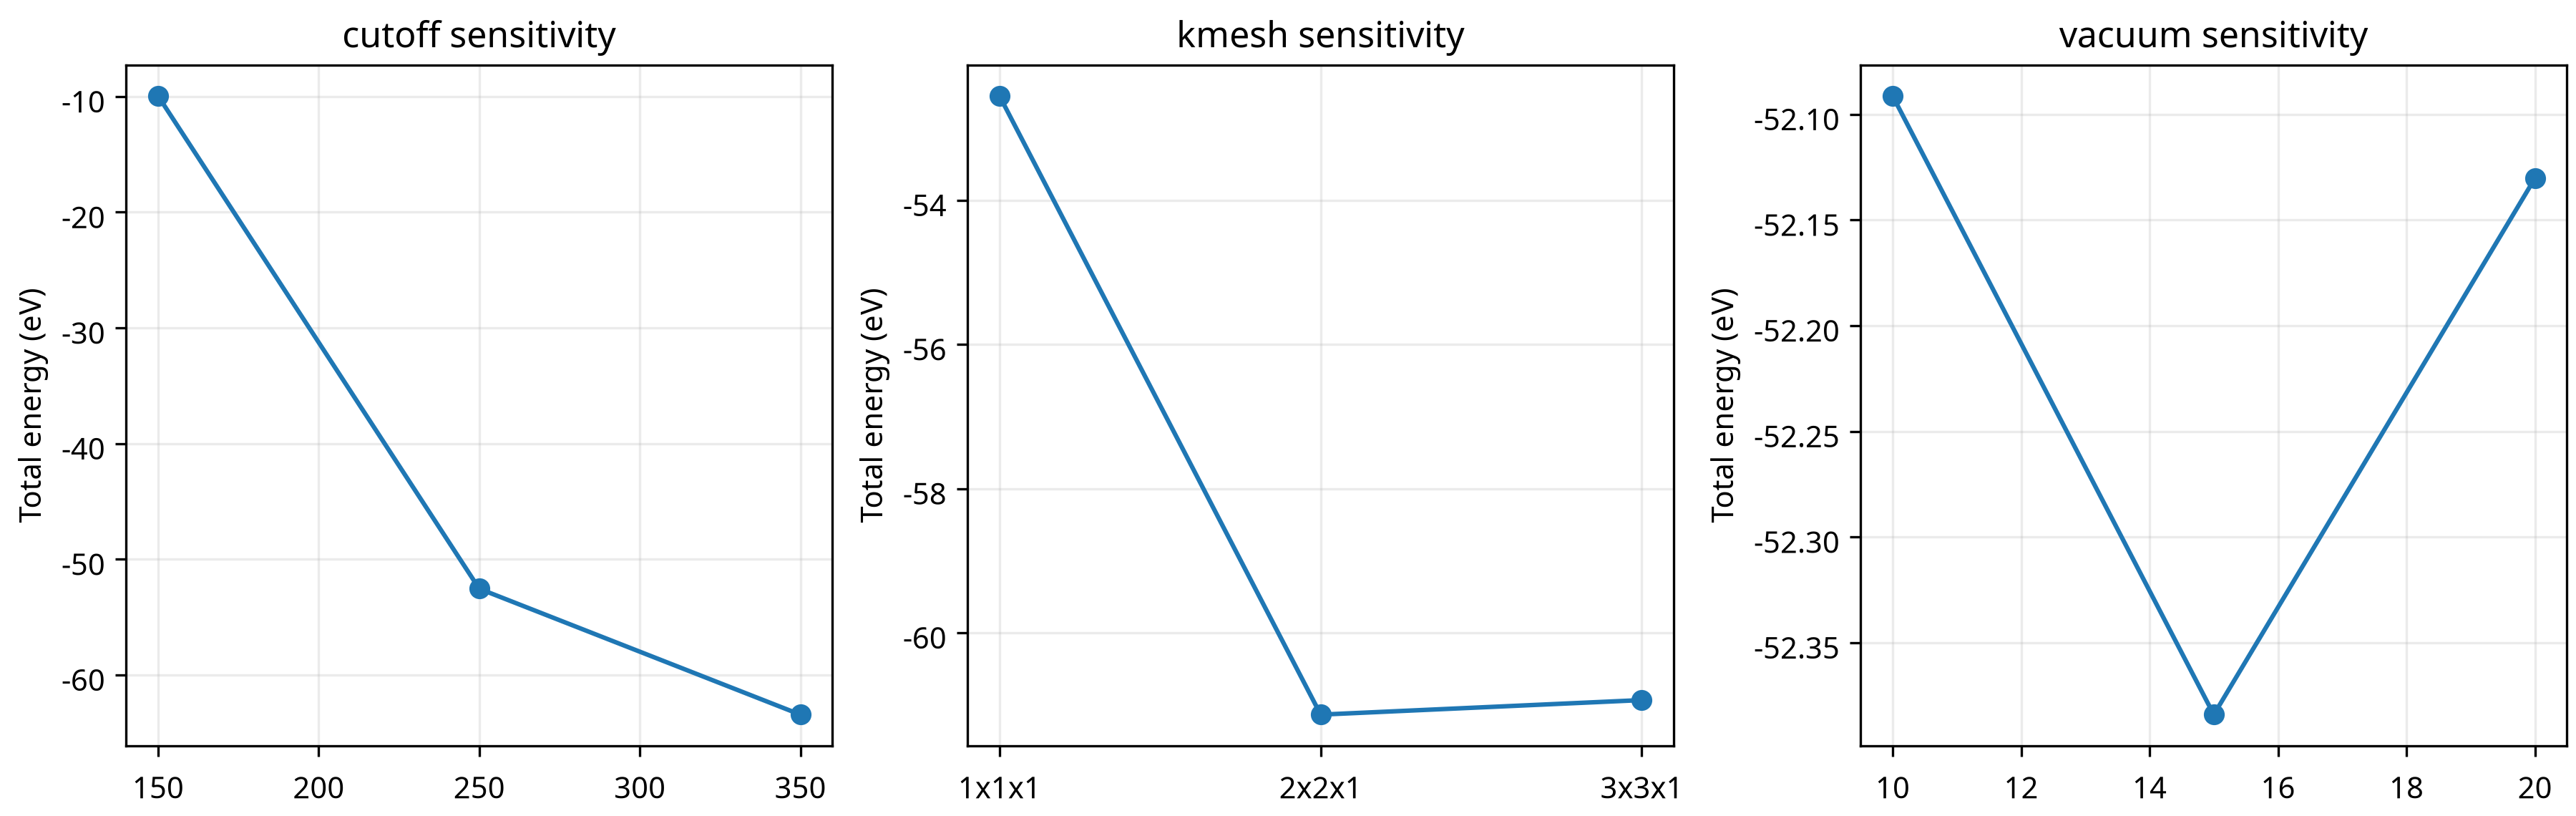
\includegraphics[width=\linewidth]{../figures/final/convergence_benchmark.png}
\caption{Compact periodic graphene convergence benchmark. The figure is diagnostic; production settings require energy-difference convergence for the actual slab and adsorbate systems.}
\end{figure}
\section{Limitations}
The complete 30-model optimisation matrix, charged-nitrate solvation corrections, transition states, free-energy diagrams, stability metrics, selectivity analysis, and catalyst ranking require substantially greater computational resources than the present sandbox. These quantities are therefore not reported as completed results.
\section{Conclusions}
A traceable open-source periodic-DFT framework was established, and the structure-generation, convergence, and audit stages were executed. The primary outcome is a reproducible baseline that prevents unsupported activity claims until the remaining calculations are performed under converged and explicitly documented conditions.
\begin{thebibliography}{5}
\bibitem{Wu2021} Wu et al., ``Electrochemical ammonia synthesis via nitrate reduction on Fe single atom catalyst,'' Nature Communications (2021). \url{https://doi.org/10.1038/s41467-021-23115-x}
\bibitem{Fan2022} Fan et al., ``Active hydrogen boosts electrochemical nitrate reduction to ammonia,'' Nature Communications (2022). \url{https://doi.org/10.1038/s41467-022-35664-w}
\bibitem{Subhadarshini2024} Subhadarshini and Pumera, ``Single Atom Catalyst for Nitrate-to-Ammonia Electrochemistry,'' Small (2024). \url{https://doi.org/10.1002/smll.202403515}
\bibitem{Sweeney2025} Sweeney, Tran, and Goldsmith, ``A grand canonical study of the potential dependence of nitrate adsorption and dissociation across metals and dilute alloys,'' Communications Chemistry (2025). \url{https://doi.org/10.1038/s42004-025-01579-y}
\end{thebibliography}
\end{document}
